\section{Methodology and Data}
\subsection{Methodologie der Arbeit}
Als Daten wurden die Bundestagsprotokolle im Zeitraum von 2009 bis 2018 von der Bundestagswebsite\thanks {https://www.bundestag.de/service/opendatav}  heruntergeladen und in einen R Datensatz eingelesen. Die Daten der Bundestagsprotokolle vor 2017 mussten mit Hilfe von regulären Ausdrücken in den Datensatz eingelesen werden, da der Inhalt der Protokolle nicht mit XML-Nodes aufgegliedert ist. Dafür wurde auch die Stammdatendatei der Politiker im Bundestag verwendet, um die Namen der Politiker als Redner in den entsprechenden Legislaturperioden identifizieren zu können. Die folgende Funktion beispielsweise teilt den Text in Reden ein, indem Sie nach dem Muster sucht, dass dem einer Rede entspricht. Dieses Muster ist für alle Protokolle gegeben durch den Namen von einem Politiker gefolgt von seiner Partei in Klammern und einem Doppelpunkt, oder der Name von einem Politiker gefolgt von einem Doppelpunkt, wenn dieser keiner Partei angehört.
\begin{verbatim}
str_split(text, paste0(c("(?<=.)(?=(",namenregex,")(?=(:| (\\(.{1,40}\\):))))")
,collapse = ""))
\end{verbatim}
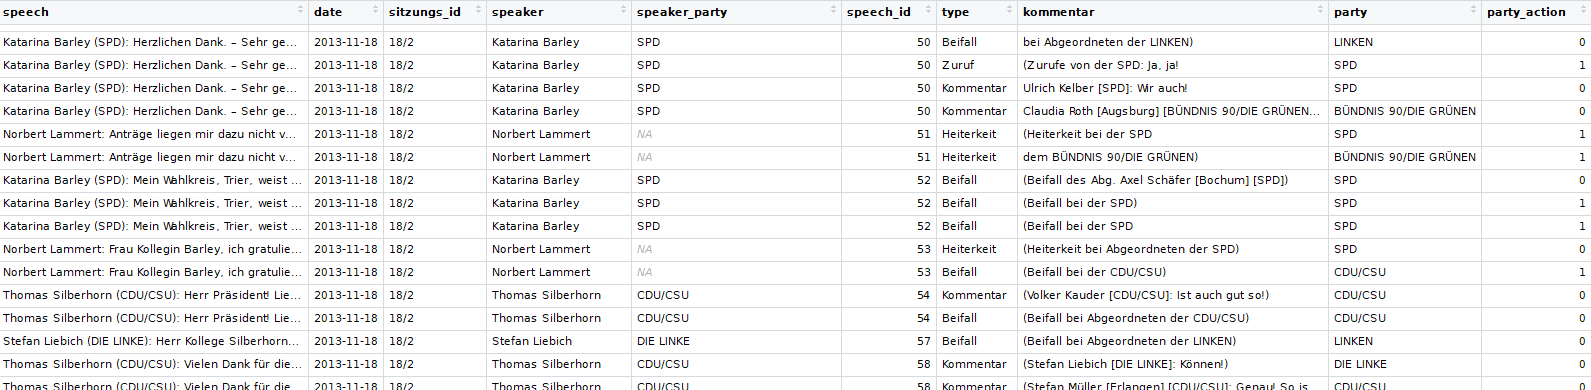
\includegraphics[width=\linewidth]{Grafiken/Head_Reden.PNG}
\\

\subsection{Methodologie der Hypothesen}
{\bfseries Hypothese 1:} Zur Überprüfung dieser Hypothese wurde eine Stichprobe aus den Plenarprotokollen gezogen, die anschließend von Hand kodiert wurde. Für eine Vergleichbarkeit der Ergebnisse besteht die Stichprobe aus jeweils 60 Reden, die in dem ersten Jahr nach Beginn der Legislaturperiode abgehalten wurden. Die Stichprobe wurde in zwei Schritten erstellt: Aus jedem Zeitraum wurden 59 Plenarprotokolle ausgewählt, das sind 2017 alle Protokolle, 2013 eine Auswahl aus 60 und 2009 eine Auswahl aus 67 Protokollen. Aus jeder der 60 Plenarprotokollen wurde eine Rede zufällig ausgewählt und den Kodierern zufällig zugeteilt. Zusätzlich wurden 10 Reden pro Kodierer auf zwei weitere Kodierer aufgeteilt, die einem späteren Reliabilitätstest dienen. Ein Beispiel für die Stichprobe:  \\
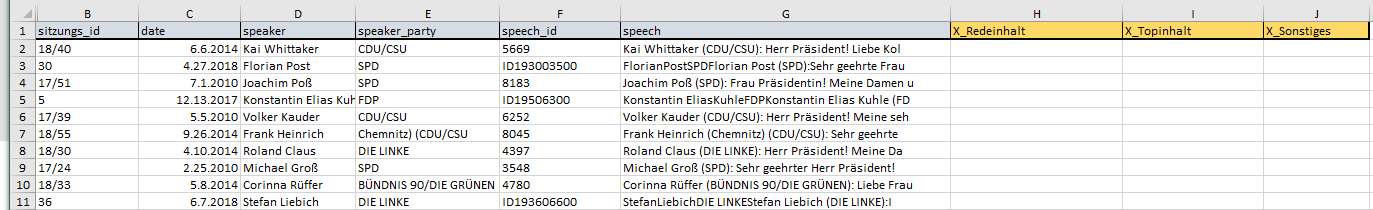
\includegraphics[width=\linewidth]{Grafiken/Head_Stichprobe.PNG}\\

{\bfseries Hypothese 2:} Zur Überprüfung der Sprachverständlichkeit wurden alle \verb 48.919  Reden im Zeitraum von 2009 bis 2017 analysiert. Für jeden Monat wurden alle Reden jeder einzelnen Partei pro Monat gruppiert und anschließend, in Silben, Wörter und Sätze aufgegliedert. Aus diesen Daten wurde der FLESCH-Index berechnet, einer der etabliertesten Readability-Indizes in der Sprachverständlichkeitsforschung. \\
{\bfseries Hypothese 3:} Zur Überprüfung der Hypothese, welche Partei wie isoliert ist, wurden alle \verb 445.301  Interaktionen im Bundestag im Zeitraum von 2009-2017 analysiert. Zusätzlich wurden die häufigsten verwendeten Wörter der Parteien analysiert. \\
{\bfseries Hypothese 4:} 
Kombination aus qualitativer Untersuchung von Kommentaren in ihren jeweiligen Reden-Kontext und die quantitative Untersuchung von stilistischen Merkmalen sprachlicher Veränderung. 


\newpage